\section{Literature Review}\label{sec:literature_review}

This literature review will provide an overview of the current state of \ac{NGS} technology, highlight the evolving key challenges for information technology, and evaluate the existing body of knowledge on \ac{SWfMS} to build a foundation for the research presented in this thesis.

\subsection{Reference Genome}
Initially, the switch to a newer reference genome is examined, as it is the fundamental change resulting in the problem at hand. This has been discussed by several journal articles. \citeauthor{Schneider2017} \autocite{Schneider2017} conclude that the current iteration of the reference genome, \textit{GRCh38}, has seen significant improvements in its assembly statistics and contains accurate representations of important clinical regions. The addition of new sequence content not only fills gaps in previous genomic data, but also captures population genomic diversity. These improvements to the assembly make \textit{GRCh38} an ideal substrate for annotation and a more effective mapping target. They recommend that \textit{GRCh38} should be utilized for all types of analyses as it represents the most comprehensive and accurate depiction of the human genome to date, surpassing previous assembly versions. \citeauthor{Guo2017} \autocite{Guo2017} compared 30 whole-exome sequencing samples processed each with \textit{GRCh37} and \textit{GRCh38}, respectively, and found that based on the comparative exome sequencing data analysis conducted between \textit{GRCh37} and \textit{GRCh38}, it can be concluded that \textit{GRCh38} represents an improvement over \textit{GRCh37}. These improvements have resulted in more accurate results for genomic analysis. \citeauthor{Pan2019} \autocite{Pan2019} describe why the change to \textit{GRCh38} should not be done by simply converting the current analyzation results to the new nomenclature, but a reanalyzation is needed, as a substantial percentage of \acp{SNV} failed to be converted during the process: approximately \SI{5}{\percent} when using \textit{GRCh38} and \SI{1}{\percent} when using \textit{GRCh37}. This observation suggests that \textit{GRCh37}, the older version, lacks some genomic resolution compared to the newer version. After conducting a thorough comparative analysis, they recommend that \textit{GRCh38} should be utilized in future SNV analysis as it presents a more advantageous option.

\subsection{Genetic Sequencing}\label{subsection:literaturegeneticsequencing}
In order to understand the fundamentals of genetic sequencing, the articles by \citeauthor{Lander2001} \autocite{Lander2001} and \citeauthor{Venter2001} \autocite{Venter2001} about the generation, assembly, and evaluation of the first whole sequence of the human genome by the \textit{Human Genome Project} give meaningful insights. The Illumina sequencer used by the \ac{DoHG@MHH} works with the \ac{NGS} technology called sequencing-by-synthesis, which was described \citeyear{Mardis2008a} by \citeauthor{Mardis2008a} \autocite{Mardis2008a}: \enquote{Cluster strands created by bridge amplification are primed and all four fluorescently labeled, 3′-OH blocked nucleotides are added to the flow cell with DNA polymerase. The cluster strands are extended by one nucleotide. Following the incorporation step, the unused nucleotides and DNA polymerase molecules are washed away, a scan buffer is added to the flow cell, and the optics system scans each lane of the flow cell by imaging units called tiles} (illustrated in \cref{figure:SBS}). It utilizes reversible terminator chemistry, demonstrated by \citeauthor{bentley2008} \autocite{bentley2008}.

The \textit{Genome in a Bottle Consortium}, hosted by the \textit{National Institute of Standards and Technology (NIST)}, provides reference data and material to calibrate, benchmark and validate the genetic analysis process. The process to produce the reference data is explained by \citeauthor{Zook2016} \autocites{Zook2016} and \citeauthor{Baid2020} \autocite{Baid2020}. Additionally, the \textit{Global Alliance for Genomics and Health (GA4GH)} provides guidelines how a genetic analysis pipeline can be benchmarked with this data, described by \citeauthor{Krusche2019} \autocite{Krusche2019}.

\begin{figure}[H]
    \centering
    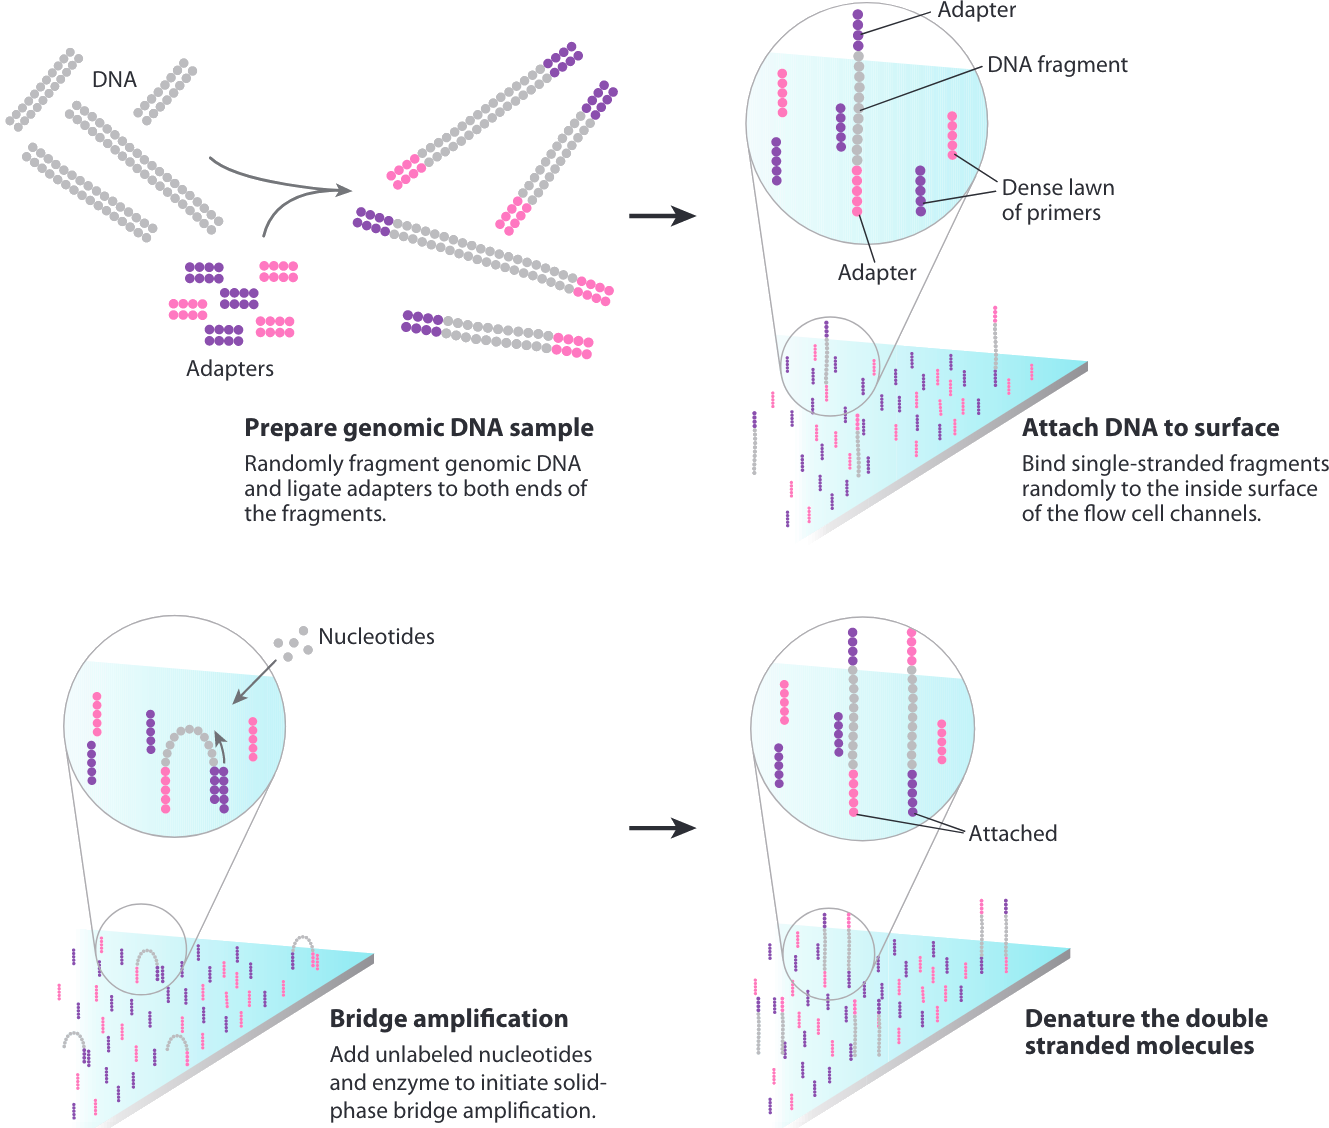
\includegraphics[width=0.9\linewidth,height=0.9\textheight,keepaspectratio]{SBS}
    \caption[The Illumina sequencing-by-synthesis approach]{The Illumina sequencing-by-synthesis approach illustrated in \autocite{Mardis2008a}}
    \label{figure:SBS}
\end{figure}

\subsection{Impact on Information Technology}
Several publications highlight the need for information technology to keep up with the advancements in \ac{NGS}: \citeauthor{Mardis2008b} discusses \citetitle{Mardis2008b} \autocite{Mardis2008b} in \citeyear{Mardis2008b} and concludes that the ongoing progress in utilizing \ac{SRS} technologies in biological research necessitates the creation of novel algorithms and software capable of accommodating the unique features of these technologies. In particular, there is a need for new tools to manage the extensive data generated by \ac{SRS} technologies and to efficiently perform common bioinformatics tasks (such as alignment) with a high volume of short reads. \citeauthor{Shendure2008} \autocite{Shendure2008} predict that the focus of the challenges will transition from acquiring proficiency in the technologies to determining the most effective methods for deriving biologically relevant or clinically significant information from massive amounts of data. \citeauthor{voelkerding2009} \autocite{voelkerding2009} foresee that over the following years, \ac{NGS} will make a successful transition into clinical diagnostics. The success of this transition will require the streamlining of processes and the ability to handle the bioinformatics challenge posed by the large amounts of sequence data output for clinical laboratories. \citeauthor{metzker2010} \autocite{metzker2010} concludes, that the generation of vast amounts of \ac{NGS} reads has presented numerous challenges for the existing information technology systems, including the difficulties in data transfer, storage, quality control, and computational analysis for read alignment and assembly. This has also placed pressure on laboratory information management systems for effective sample tracking and process management. Despite ongoing advancements in bioinformatics, it is essential to make further enhancements in order to keep up with the fast-paced developments in \ac{NGS} technologies. There is a possibility that the costs associated with the handling and analysis of NGS data could be on par or even surpass the cost of producing the data.

\subsection{Scientific Workflow Management Systems}\label{subsec:literature_review_swfms}
According to \citeauthor{georgakopoulos1995} \autocite{georgakopoulos1995}, \enquote{workflow management is a technology supporting the reengineering of business and information processes. It involves: 1. defining workflows, i.e., describing those aspects of a process that are relevant to controlling and coordinating the execution of its tasks (and possibly the skills of individuals or information systems required to perform each task), and 2. providing for fast (re)design and (re)implementation of the processes as business needs and information systems change}. \citeauthor{aalst2004} \autocite{georgakopoulos1995} define a \ac{WfMS} as typically composed of three main components: a workflow model, a workflow engine, and a workflow repository. The workflow model defines the steps and tasks involved in a workflow, the workflow engine executes the workflow, and the workflow repository stores and manages the workflow information.

Execution models of \acp{SWfMS} differentiate themselves by being data-flow oriented instead of event and control-flow driven like business workflows, in accordance with \citeauthor{ludascher2006} \autocite{ludascher2006} describing their system \textit{Kepler}. Additional \acp{SWfMS} from the early 2000s include \textit{Taverna} as described by \citeauthor{oinn2004} \autocite{oinn2004} and \textit{Galaxy} introduced by \citeauthor{giardine2005} \autocite{giardine2005}. Only \textit{Galaxy} is still maintained today.

More recent forays in the realm of \ac{SWfMS} are \textit{Snakemake} (\url{https://snakemake.github.io/}), introduced by \citeauthor{koster2012} \autocite{koster2012}, and \textit{Nextflow} (\url{https://www.nextflow.io/}), described by \citeauthor{ditommaso2017} \autocite{ditommaso2017}. \textit{Snakemake} and \textit{Nextflow} follow a similar concept. Both feature a \ac{DSL} to describe workflows in a text-based definition, which \citeauthor{koster2012} see as advantageous: workflows can be modified outside a graphical interface, such as on a remote server, and developers can collaborate on them utilizing source code management tools. There are differences in details, but they are nevertheless relevant for the \ac{DoHG@MHH}. The \ac{HPC} cluster is managed with \textit{\ac{SLURM}}, so direct support is preferred. As the use of cloud infrastructure should be evaluated, \ac{AWS} support is required. \Cref{tab:nextflow_vs_snakemake} shows that \textit{Snakemake} is lacking in these crucial areas. \citeauthor{ditommaso2017} further note that the task sequence in \textit{Snakemake} is determined by rules and patterns based on the input and output file names, which makes it challenging to manage multiple dynamically generated output files, leading to the need for the implementation of low-level output management procedures. However, \textit{Nextflow} enables the use of any data structure, and its outputs are not limited to files but can also include in-memory values and data objects. Unlike \textit{Snakemake}, which requires a \ac{DAG} to store the task execution order, \textit{Nextflow} uses a top to bottom processing model, which follows the natural flow of data analysis. This approach does not require pre-computing or storing a \ac{DAG}, resulting in high scalability and making it suitable for large computational tasks. Compared to \textit{Galaxy}, \citeauthor{ditommaso2017} note that the \ac{GUI}, which provides robust support for non-specialists to implement \textit{de novo} pipelines, also places a substantial development load as any pre-existing and validated third-party pipeline must be recreated and reconfigured using the \ac{GUI}.

\textit{Nextflow} was chosen by a group of \~{}25 Computational Biologists and Data Scientists at the \textit{September 2017 Pitt-NCBI Hackathon} to create a proof-of-principle simple RNA-seq pipeline at \autocite{poholek2017}. \textit{Snakemake} was discarded due to its inflexibility compared to \textit{Nextflow}. \textit{Nextflow} was ultimately selected because of its ability to utilize any programming language, handle inputs and outputs effectively, and its ease of wrapping. The authors also highlight its usefulness and versatility in their report. \citeauthor{larsonneur2018} \autocite{larsonneur2018} present benchmarks for several \acp{SWfMS}, and find that \textit{Snakemake} and \textit{Nextflow} showed close performances. \citeauthor{jackson2021} \autocite{jackson2021} use prototyping to find a suitable \ac{SWfMS} to wrap their existing pipeline, \textit{RiboViz}, and chose \textit{Nextflow} for several reasons. The ability to execute each step within separate subdirectories and the option to re-execute individual steps is useful for debugging purposes. Although writing in \textit{Groovy} is required to develop workflows in \textit{Nextflow}, the authors, who had prior experience with \textit{Python} and \textit{R}, found learning \textit{Groovy} to be manageable. Additionally, the built-in support and comprehensive documentation for containers, high-performance computing systems, and cloud platforms offered by \textit{Nextflow} appeared to be more extensive than those provided by \textit{Snakemake}. They conclude that they can use \textit{Nextflow} to construct \textit{RiboViz} in a more portable and maintainable manner, enabling them to take advantage of the power of distributed computing resources to analyze large-scale datasets. \citeauthor{wratten2021} \autocite{wratten2021} compare several \acp{SWfMS} and give \textit{Nextflow} the highest marks over several categories as shown in \cref{tab:wratten2021}. They also highlight the \textit{nf-core} framework for \textit{Nextflow} introduced by \citeauthor{ewels2020} \autocite{ewels2020} as collaboratively created best-practice analytic pipelines that are peer-reviewed by the community, which might prove useful for future endeavors at the \ac{DoHG@MHH}. \citeauthor{Ahmed2021} \autocite{Ahmed2021} benchmark \textit{Nextflow} against \textit{Swift/T}, \textit{CWL} and \textit{WDL}. They observe that \textit{Nextflow} scales particularly well, sometimes outperforming the other tools fifty-fold. The other categories examined (modularity, robustness, reproducibility, portability, interoperability, and ease of development) show differences between the tools, with \textit{Nextflow} fulfilling all of these satisfactorily.

\begin{table}[H]
\centering
\begin{threeparttable}[c]
\caption{Comparison of Nextflow with other workflow management systems\tnote{a}}
\label{tab:nextflow_vs_snakemake}
\begin{tabular}{lccc}
\toprule
\acs{SWfMS} & Nextflow & Snakemake & Galaxy \\ \midrule
Platform & Groovy/JVM & Python & Python \\
Workflow versioning & Yes & No & Yes \\
Automatic error failover & Yes & No & No \\
SLURM support & Yes & Partial & Yes \\
AWS support & Yes & No & Yes \\
\bottomrule
\end{tabular}
\begin{tablenotes}
\footnotesize{\item[a]Excerpt from \autocite[Table 1]{ditommaso2017}}
\end{tablenotes}
\end{threeparttable}
\end{table}

\begin{table}[H]
\centering
\begin{threeparttable}[c]
\caption{Overview of workflow managers for bioinformatics\tnote{a}}
\label{tab:wratten2021}
\begin{tabular}{lccccccc}
\toprule
 & {\rotatebox[origin=c]{90}{Ease of Use}} & {\rotatebox[origin=c]{90}{Expressiveness}} & {\rotatebox[origin=c]{90}{Portability}} & {\rotatebox[origin=c]{90}{Scalability}} & {\rotatebox[origin=c]{90}{Learning Resources}} & {\rotatebox[origin=c]{90}{Pipeline Initiatives}} & {\rotatebox[origin=c]{90}{Sum}} \\ \midrule
Galaxy & 3 & 1 & 3 & 3 & 3 & 2 & 15 \\
Nextflow & 2 & 3 & 3 & 3 & 3 & 3 & 17 \\
Snakemake & 2 & 3 & 2.5 & 3 & 2 & 3 & 15.5 \\
\bottomrule
\end{tabular}
\begin{tablenotes}
\footnotesize{\item[a]Excerpt from \autocite[Table 1]{wratten2021}}
\end{tablenotes}
\end{threeparttable}
\end{table}